\documentclass[usenames,dvipsnames,10pt]{beamer}
\usepackage[absolute,overlay]{textpos}

% Setup appearance:
\usetheme{Boadilla}
\usefonttheme[onlylarge]{structurebold}
\usecolortheme{seahorse}
\setbeamerfont*{frametitle}{size=\normalsize,series=\bfseries}
\setbeamertemplate{navigation symbols}{}
%\setbeamercolor{frametitle}{fg=Blue}
\renewcommand\alert[1]{{\color{Magenta} #1}}
\newcommand\program[1]{\texttt{#1}}

% Packages
\usepackage[english,ukrainian]{babel}
\usepackage{times}
\usepackage[T1]{fontenc}
\usepackage{color}
\usepackage{bm}
\usepackage{slashed}
\usepackage{booktabs}% http://ctan.org/pkg/booktabs
\usepackage{xspace}
\usepackage{multirow}
\usepackage{graphicx}
\newcommand{\tabitem}{~~\llap{\textbullet}~~}
\usepackage{minted}
\usepackage{scalerel}
\usepackage{amsmath}

\hypersetup{
	colorlinks=true,
	linktoc=page,
	citecolor=Blue,
	linkcolor=Blue,
	urlcolor=Blue 
}

\setlength{\fboxsep}{0pt}%
\setlength{\fboxrule}{1pt}%

%\definecolor{stcoupcolor}{RGB}{255,0,51}

% Setup TikZ
\usepackage{tikz}
\usetikzlibrary{arrows,shapes,backgrounds,positioning}
\tikzstyle{block}=[draw opacity=0.7,line width=1.4cm]

% arrows
\tikzset{
    myarrow/.style={
        draw,
        fill=orange,
        single arrow,
        rounded corners=1,
        %        width=2ex,
        minimum width=2ex,
        minimum height=3ex,
        single arrow head extend=1ex
    }
}
\newcommand{\arrowup}{\tikz [baseline=-0.5ex]{\node [myarrow,rotate=90] {};}}
\newcommand{\arrowdown}{\tikz [baseline=-0.5ex]{\node [myarrow,rotate=-90] {};}}
\newcommand{\arrowright}{\tikz [baseline=-0.5ex]{\node [myarrow,rotate=0] {};}}
\newcommand{\arrowleft}{\tikz [baseline=-0.5ex]{\node [myarrow,rotate=180] {};}}

% draw connection
\newcommand{\tikzmark}[1]{\tikz[remember picture] \node[coordinate] (#1) {#1};}

% page numbering (backup)
\newcommand{\backupbegin}{\newcounter{finalframe}\setcounter{finalframe}{\value{framenumber}}}
\newcommand{\backupend}{\setcounter{framenumber}{\value{finalframe}}}

% Author, Title, etc.
\title[CMS Open Data]{\large Вимірювання диференційних перерізів народження $t\bar{t}$ з використання CMS Open Data}
\author[Олександр Зенаєв]{Олександр Зенаєв}
\date{}

% block with custom width
\newenvironment<>{varblock}[2][.9\textwidth]{%
    \setlength{\textwidth}{#1}
    \begin{actionenv}#3%
        \def\insertblocktitle{#2}%
        \par%
        \usebeamertemplate{block begin}}
    {\par%
        \usebeamertemplate{block end}%
\end{actionenv}}

\setbeamertemplate{itemize/enumerate body begin}{\footnotesize}
\setbeamertemplate{itemize/enumerate subbody begin}{\footnotesize}

\tikzset{
    every overlay node/.style={
        rounded corners,anchor=north west,
    },
}
\def\tikzoverlay{%
    \tikz[baseline,overlay]\node[every overlay node]
}%

% main part
\begin{document}
    \begin{frame}[plain]
    %\centering\includegraphics[width=0.15\textwidth]{pics/logo/cms.png}
    %\hspace{0.1\textwidth}
    %\centering\includegraphics[width=0.18\textwidth]{pics/logo/h1}
    %\hspace{0.1\textwidth}
    %\centering\includegraphics[width=0.15\textwidth]{pics/logo/desyNEW}
    %\hspace{0.1\textwidth}
    %\centering\includegraphics[width=0.15\textwidth]{pics/logo/zeus}
    %\hspace{0.1\textwidth}
    %\centering\includegraphics[width=0.15\textwidth]{pics/logo/xFitterLogo1.png}
    
    \vspace{-0.05\textheight}
    \titlepage
    
    %\vspace{-0.15\textheight}
    %\centering\includegraphics[width=0.4\textwidth]{pics/titlepic.jpg}

    %\vspace{-0.15\textheight}
    %{\color{blue} Overview:}
    
    \vspace{0.04\textheight}
    \centering
    %place \\
    %date
\end{frame}

% number of slides w/out backup
\renewcommand{\inserttotalframenumber}{2}
\setbeamercolor{footline}{fg=blue}
\setbeamerfont{footline}{series=\bfseries}


\begin{frame}
\frametitle{Стандартна модель (СМ)}
\begin{columns}\column{\dimexpr\paperwidth-10pt}
\begin{columns}
	\column{0.65\textwidth}
	\centering{\includegraphics[width=1.0\textwidth]{pics/SM\_particles-001.png}}
	\column{0.35\textwidth}
	\begin{itemize}
		\item Топ кварк ($t$) є найважчою  елементарною частинкою в Стандартній Моделі
		\item Tevatron (Fermilab) і LHC (CERN)
		\item Дослідження процесів з топ кварками (перерізи народження і властивості) дозволяє перевірити/покращити існуючі теоретичні моделі і створити/спростувати нові моделі
	\end{itemize}
\end{columns}
\end{columns}
\end{frame}

\begin{frame}
	\frametitle{Народження топ кварків у зіткненнях протонів}
\begin{columns}
	\column{0.3\textwidth}
	\centering{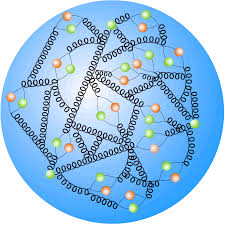
\includegraphics[width=0.7\textwidth]{pics/pdfs.jpeg}}
	\centering{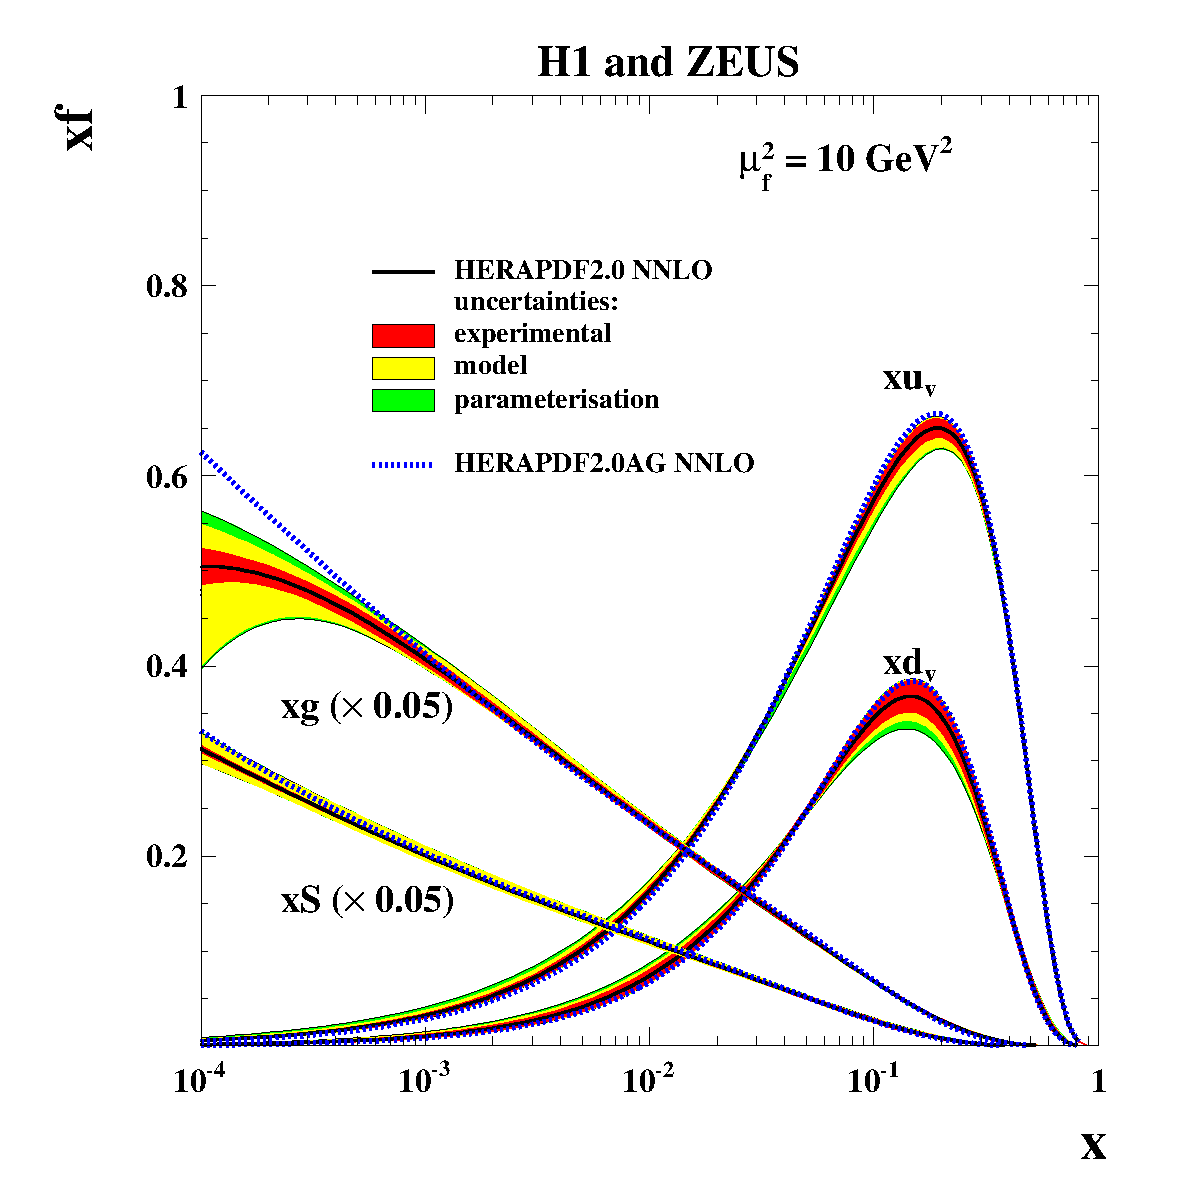
\includegraphics[width=1.0\textwidth]{pics/d15-039f23.pdf}}
	\centering{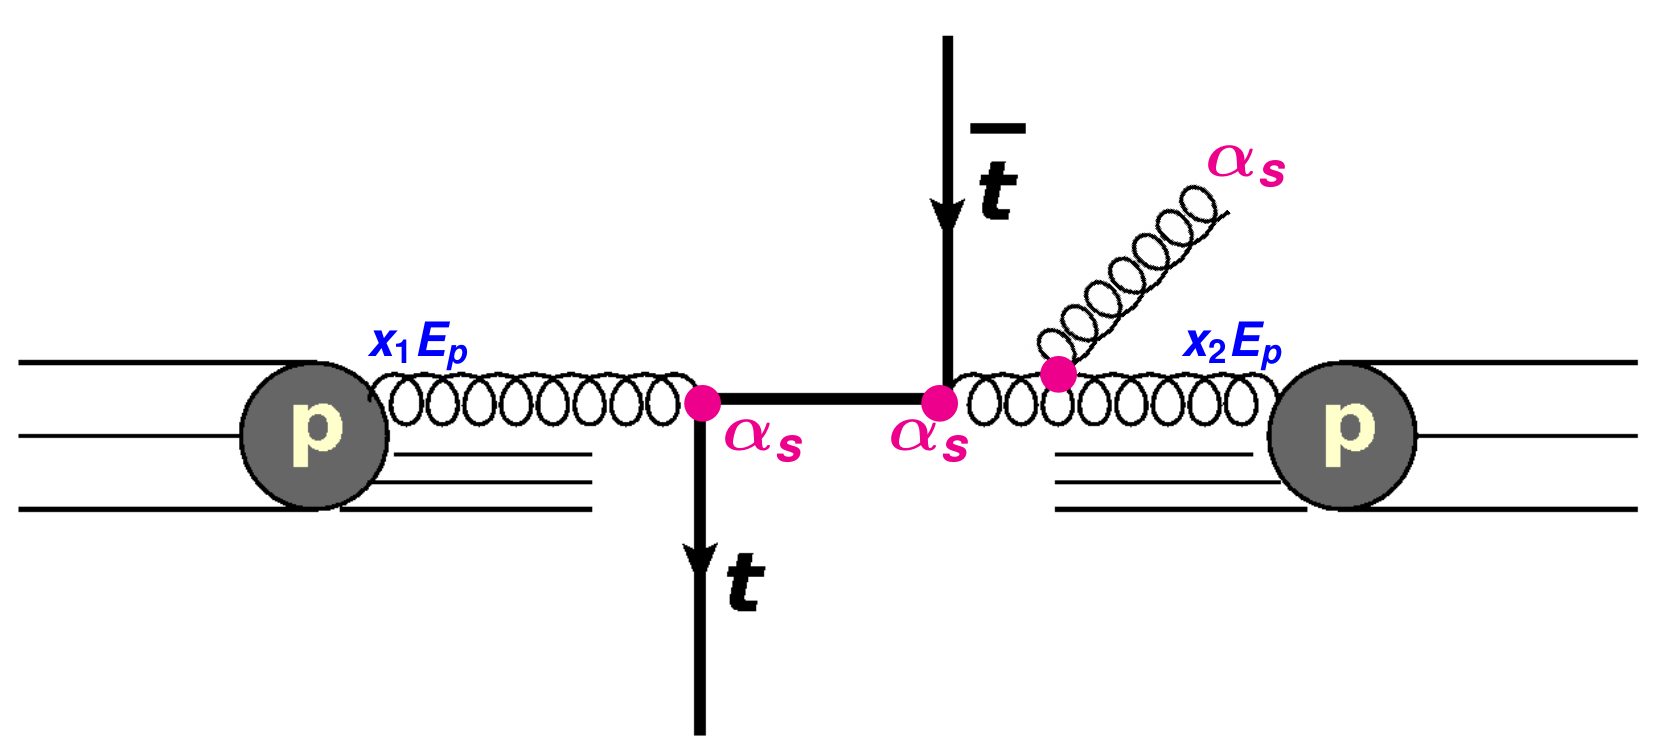
\includegraphics[width=1.3\textwidth]{pics/scr-tt-sz.png}}
	\column{0.7\textwidth}
	\begin{itemize}
		\item Протон складається з uud кварків що взаємодію через обмін глюонів: густина розподілу партонів (parton distribution functions, PDFs)
		\item Квантова хромодинаміка (Quantum Chromodynamics, QCD) описує сильну взаємодію кварків і глюонів
		\item Пертербутавний режим (теорія збурень): $\alpha_S(\mu) < 1$, $\mu \sim 1$ GeV$ \gg \Lambda_{QCD}$
		\item $\sigma = \Sigma_{i=0}^n \sigma_i \alpha_S^i$
		\item PDFs параметризують непертурбативну фізику; на даний момент їх не обчислюють, а визначають з експериментальних даних: $f_{q,\bar{q},g}(\mu,x)$
		\item Дані з народження топ кварків є суттєвим джерелом інформації про глюонні PDFs за великих значень $x$ (важливо для пошуків нової фізики)
		\item Також з перерізів народження топ кварків визначають $\alpha_S$ і $m_t$ (вільні параметри СМ)
	\end{itemize}
	
	\vspace{0.1\textheight}
\end{columns}
\end{frame}

\begin{frame}
	\frametitle{CMS Open Data}
	\begin{itemize}
		\item \url{https://cms-opendata-guide.web.cern.ch/}
		\item Репозиторії з прикладами:
		\begin{itemize}
			\item \url{https://github.com/cms-opendata-validation}
			\item \url{https://github.com/cms-opendata-analyses}
		\end{itemize}
		\item Зазвичай аналіз містить дві частини:
		\begin{itemize}
			\item обробка ``сирих'' CMS даних з використанням CMS software (CMSSW) і створення ROOT нтуплів [Analyzer]
			\item[] $\to$ RECO, AOD, MiniAOD, NanoAOD \dots
			\item[] $\to$ потрібний значний CPU ресурс та інтернет трафік (зазвичай використовують комп'ютерний кластер)
			\item обробка ROOT нтуплів (без CMSSW) [PostAnalyzer]
			\item[] $\to$ можна працювати на будь-якому комп'ютері (хвилини або секунди)
		\end{itemize}
	\end{itemize}
\end{frame}

\begin{frame}[fragile]
	\frametitle{Практичне завдання: обробка CMS AOD даних за 2011 рік [Analyzer]}
	\begin{itemize}
		\item \url{https://cms-opendata-guide.web.cern.ch/}
		\item Перший раз завантажити контейнер із CMS software:
	{\scriptsize
	\begin{minted}{c++}
docker run -it --name my_od --net=host --env="DISPLAY" -v \
		    $HOME/.Xauthority:/home/cmsusr/.Xauthority:rw\
		    cmsopendata/cmssw_5_3_32-slc6_amd64_gcc472 /bin/bash
exit
	\end{minted}
	}
		\item Наступного разу запустити контейнер:
		{\scriptsize
			\begin{minted}{c++}
docker start -i my_od
		\end{minted}
		}
		\item Далі виконувати інструкції для Analyzer із \newline \url{https://github.com/zenaiev/2011-ttbar} \newline і запустити Analyzer для одного файлу з даними і МК
	\end{itemize}
\end{frame}

%\appendix
%\backupbegin
%\begin{frame}
%\frametitle{}
%\centering{\Huge \bf BACKUP}
%\end{frame}
%\backupend

\end{document}
